\documentclass{article}
\usepackage[utf8]{inputenc}
\usepackage[greek,english]{babel}
\usepackage{alphabeta}
\usepackage{fancyhdr}
\usepackage{listings}
\usepackage{mathtools}
\usepackage{xcolor}
\usepackage{biblatex}
\usepackage[left=2cm,right=2cm]{geometry}

\lstset {
        basicstyle=\ttfamily,
        columns=fullflexible,
        breaklines=true,
        keepspaces=true,
	showstringspaces=false
}

\title{Εργαστήριο Κατανεμημένων Συστημάτων - Εργασία 1}
\author{Χρήστος Μαργιώλης -- 19390133}
\date{Μάιος 2022}

\begin{document}

\begin{titlepage}
        \maketitle
        \begin{figure}[t!]
        \begin{center}
        
\includegraphics[scale=0.3]{./res/uniwalogo.png} \\
        \Large
        \textbf{Πανεπιστήμιο Δυτικής Αττικής} \\
        \large
        Τμήμα Μηχανικών Πληροφορικής και Ηλεκτρονικών Υπολογιστών
        \end{center}
        \end{figure}
\end{titlepage}

\renewcommand{\contentsname}{Περιεχόμενα}
\tableofcontents

\section{Χρήση \lstinline{rpcgen}}

Πριν γίνει η ανάπτυξη του client/server κώδικα, πρέπει να παραχθούν τα
απαραίτητα RPC αρχεία. Στο αρχείο \lstinline{rpc.x} δηλώνονται τα ονόματα
και οι δομές των Remote Procedure Calls.

Παράγουμε τα client και server stubs (αρχεία στα οποία θα συμπληρωθεί ο
κώδικας), καθώς και το \lstinline{Makefile} για να είναι πιο εύκολη η
μεταγλώττιση:

\begin{lstlisting}
	$ rpcgen -Ss -C > rpc_server.c
	$ rpcgen -Sc -C > rpc_client.c
	$ rpcgen -Sm > Makefile.rpc
\end{lstlisting}

Στο \lstinline{Makefile.rpc} κάνουμε μερικές αλλαγές ωστέ ο server να μην
τρέχει στο background, και στην μεταγλώττιση να περιέχονται τα
\lstinline{rpc_client.c} και \lstinline{rpc_server.c}:

\begin{lstlisting}[language=make]
	...
	TARGETS_SVC.c = rpc_server.c rpc_svc.c rpc_xdr.c
	TARGETS_CLNT.c = rpc_client.c rpc_clnt.c rpc_xdr.c
	...
	CFLAGS += -g -DRPC_SVC_FG
	RPCGENFLAGS = -C
\end{lstlisting}

\section{Εκτέλεση κώδικα}

Το αρχείο \lstinline{sock_client.c} υλοποιεί τον client τον οποίο εκτελεί ο
χρήστης. Το \lstinline{rpc_client.c}, παρόλο που λέει "client", είναι ο server
με τον οποίο επικοινωνεί ο \lstinline{sock_client.c} και κάνει τις remote
κλήσεις στον \lstinline{rpc_server.c}, ο οποίος υλοποιεί τις συναρτήσεις των
RPC.

Κάνουμε compile τους κώδικες:

\begin{lstlisting}
	$ make
	make -f Makefile.rpc
	rpcgen -C rpc.x
	cc  -O2 -pipe -g -DRPC_SVC_FG -c rpc_client.c -o rpc_client.o
	cc  -O2 -pipe -g -DRPC_SVC_FG -c rpc_clnt.c -o rpc_clnt.o
	cc  -O2 -pipe -g -DRPC_SVC_FG -c rpc_xdr.c -o rpc_xdr.o
	cc -o rpc_client  rpc_client.o rpc_clnt.o rpc_xdr.o  -O2 -pipe -g -DRPC_SVC_FG
	cc  -O2 -pipe -g -DRPC_SVC_FG -c rpc_server.c -o rpc_server.o
	cc  -O2 -pipe -g -DRPC_SVC_FG -c rpc_svc.c -o rpc_svc.o
	cc -o rpc_server  rpc_server.o rpc_svc.o rpc_xdr.o  -O2 -pipe -g -DRPC_SVC_FG
	cc sock_client.c -o sock_client
\end{lstlisting}

Τα τρία προγράμματα εκτελούνται ως εξής:
\begin{itemize}
	\item \lstinline{./rpc_server}
	\item \lstinline{./rpc_client [-b backlog] [-p port] hostname}
	\item \lstinline{./sock_client [-p port] hostname}
\end{itemize}

Πριν τρέξουμε οποιοδήποτε RPC πρόγραμμα, πρέπει να αρχίσουμε το
\lstinline{rpcbind(8)} service (για FreeBSD):

\begin{lstlisting}
	# service rpcbind start
\end{lstlisting}

Αφού τρέξουμε τον server, μπορούμε να δούμε ότι τα Remote Procedure Calls
έχουνε εισαχθεί στον πίνακα RPC. Η εντολή \lstinline{rpcinfo(8)} τυπώνει
τον πίνακα:

\begin{lstlisting}
	$ ./rpc_server
	$ rpcinfo
	   program version netid     address                service    owner
	    100000    4    tcp       0.0.0.0.0.111          rpcbind    superuser
	    100000    3    tcp       0.0.0.0.0.111          rpcbind    superuser
	    100000    2    tcp       0.0.0.0.0.111          rpcbind    superuser
	    100000    4    udp       0.0.0.0.0.111          rpcbind    superuser
	    100000    3    udp       0.0.0.0.0.111          rpcbind    superuser
	    100000    2    udp       0.0.0.0.0.111          rpcbind    superuser
	    100000    4    tcp6      ::.0.111               rpcbind    superuser
	    100000    3    tcp6      ::.0.111               rpcbind    superuser
	    100000    4    udp6      ::.0.111               rpcbind    superuser
	    100000    3    udp6      ::.0.111               rpcbind    superuser
	    100000    4    local     /var/run/rpcbind.sock  rpcbind    superuser
	    100000    3    local     /var/run/rpcbind.sock  rpcbind    superuser
	    100000    2    local     /var/run/rpcbind.sock  rpcbind    superuser
	 536870912    1    udp6      ::.161.100             -          1001
	 536870912    1    tcp6      ::.93.202              -          1001
	 536870912    1    udp       0.0.0.0.44.39          -          1001
	 536870912    1    tcp       0.0.0.0.219.61         -          1001
	 536870913    1    udp6      ::.161.100             -          1001
	 536870913    1    tcp6      ::.93.202              -          1001
	 536870913    1    udp       0.0.0.0.44.39          -          1001
	 536870913    1    tcp       0.0.0.0.219.61         -          1001
	 536870914    1    udp6      ::.161.100             -          1001
	 536870914    1    tcp6      ::.93.202              -          1001
	 536870914    1    udp       0.0.0.0.44.39          -          1001
	 536870914    1    tcp       0.0.0.0.219.61         -          1001
\end{lstlisting}

Οι γραμμές που ξεκινούν με 53687* είναι τα RPC που δημιούργησε ο
\lstinline{rpc_server}.

\section{Ενδεικτικά τρεξίματα}

Σε κάθε ενότητα έχω παραθέσει τα output των 3 προγραμμάτων στην τελική τους
κατάσταση. 'Ισως χρειαστεί λίγη μεγέθυνση...

\subsection{Server και client στον ίδιο υπολογιστή}

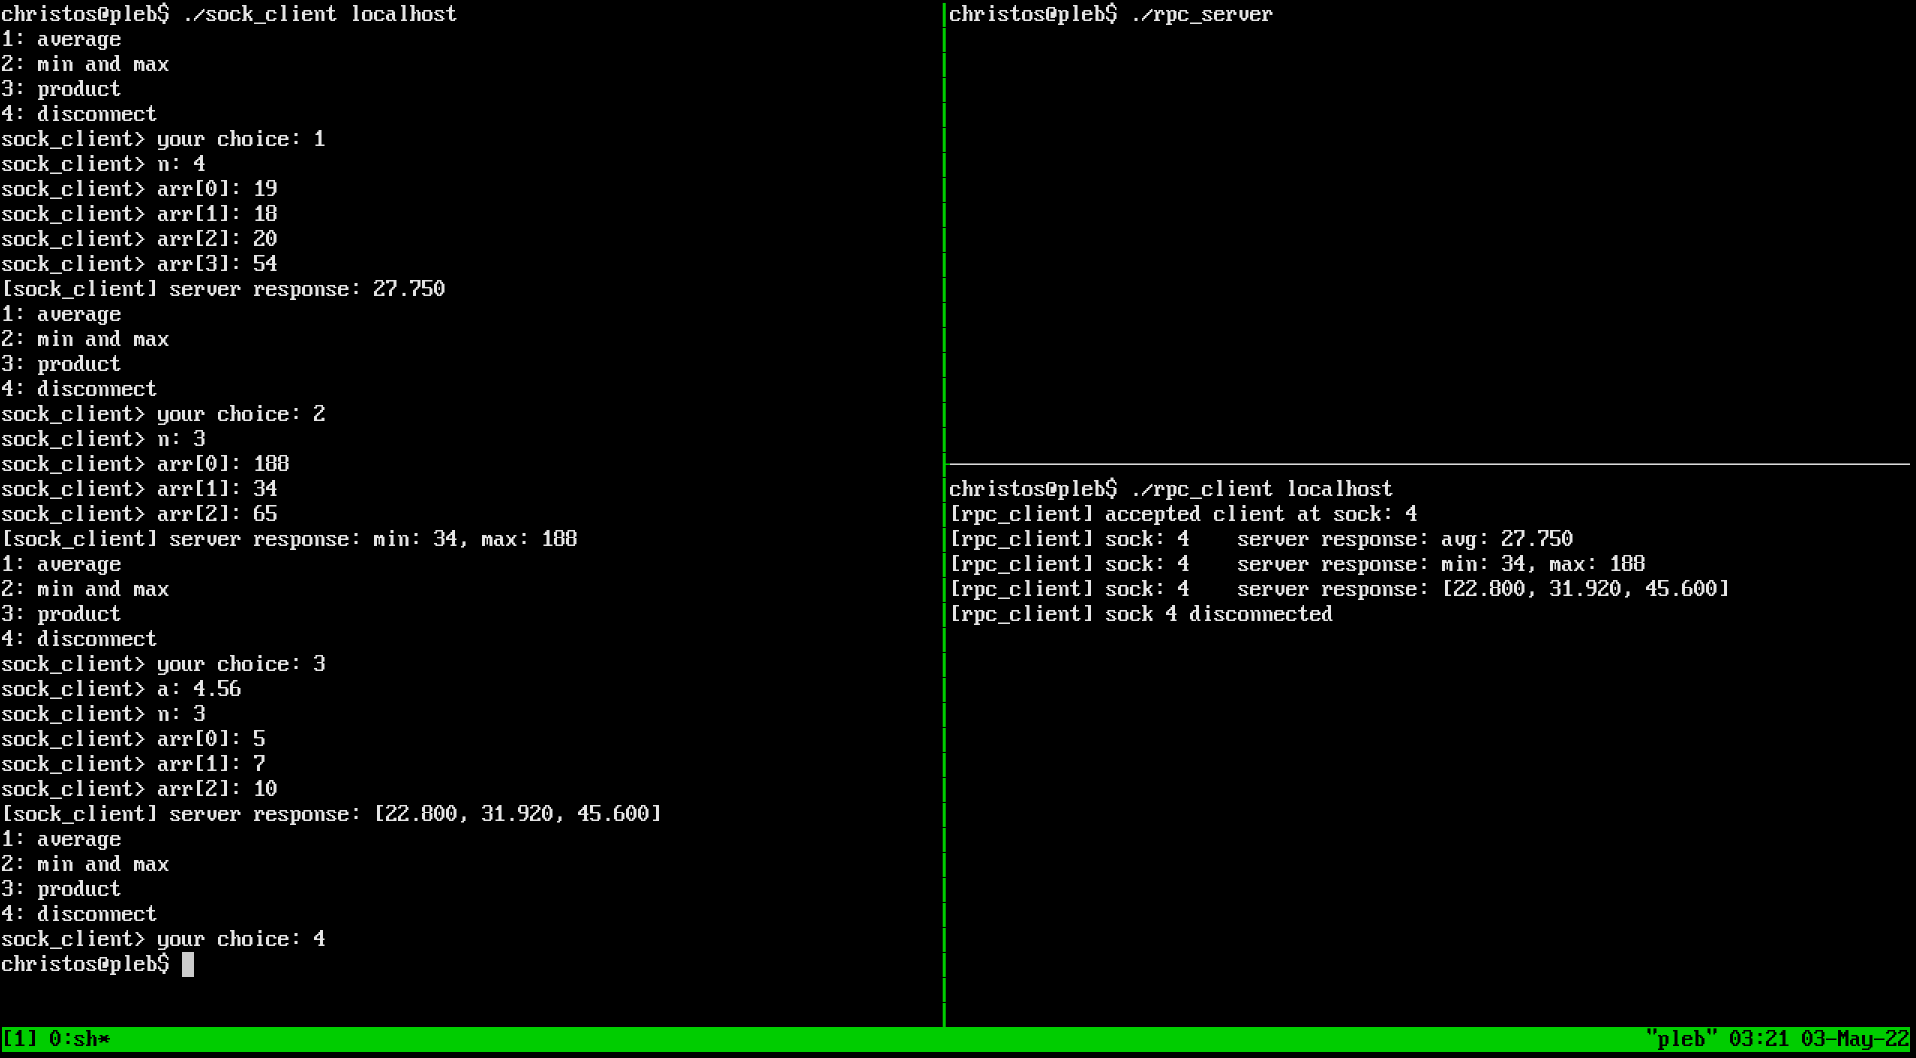
\includegraphics[width=\linewidth]{res/samepc.png}

\subsection{Server και client σε διαφορετικές IP}

Ο RPC server τώρα τρέχει σε FreeBSD Jail, το οποίο, αν και βρίσκεται στο ίδιο
τοπικό δίκτυο, έχει διαφορετική IP διεύθυνση. Ο RPC client και ο socket client
τρέχουν ακόμα στο τρέχουν ακόμα στον localhost. \\

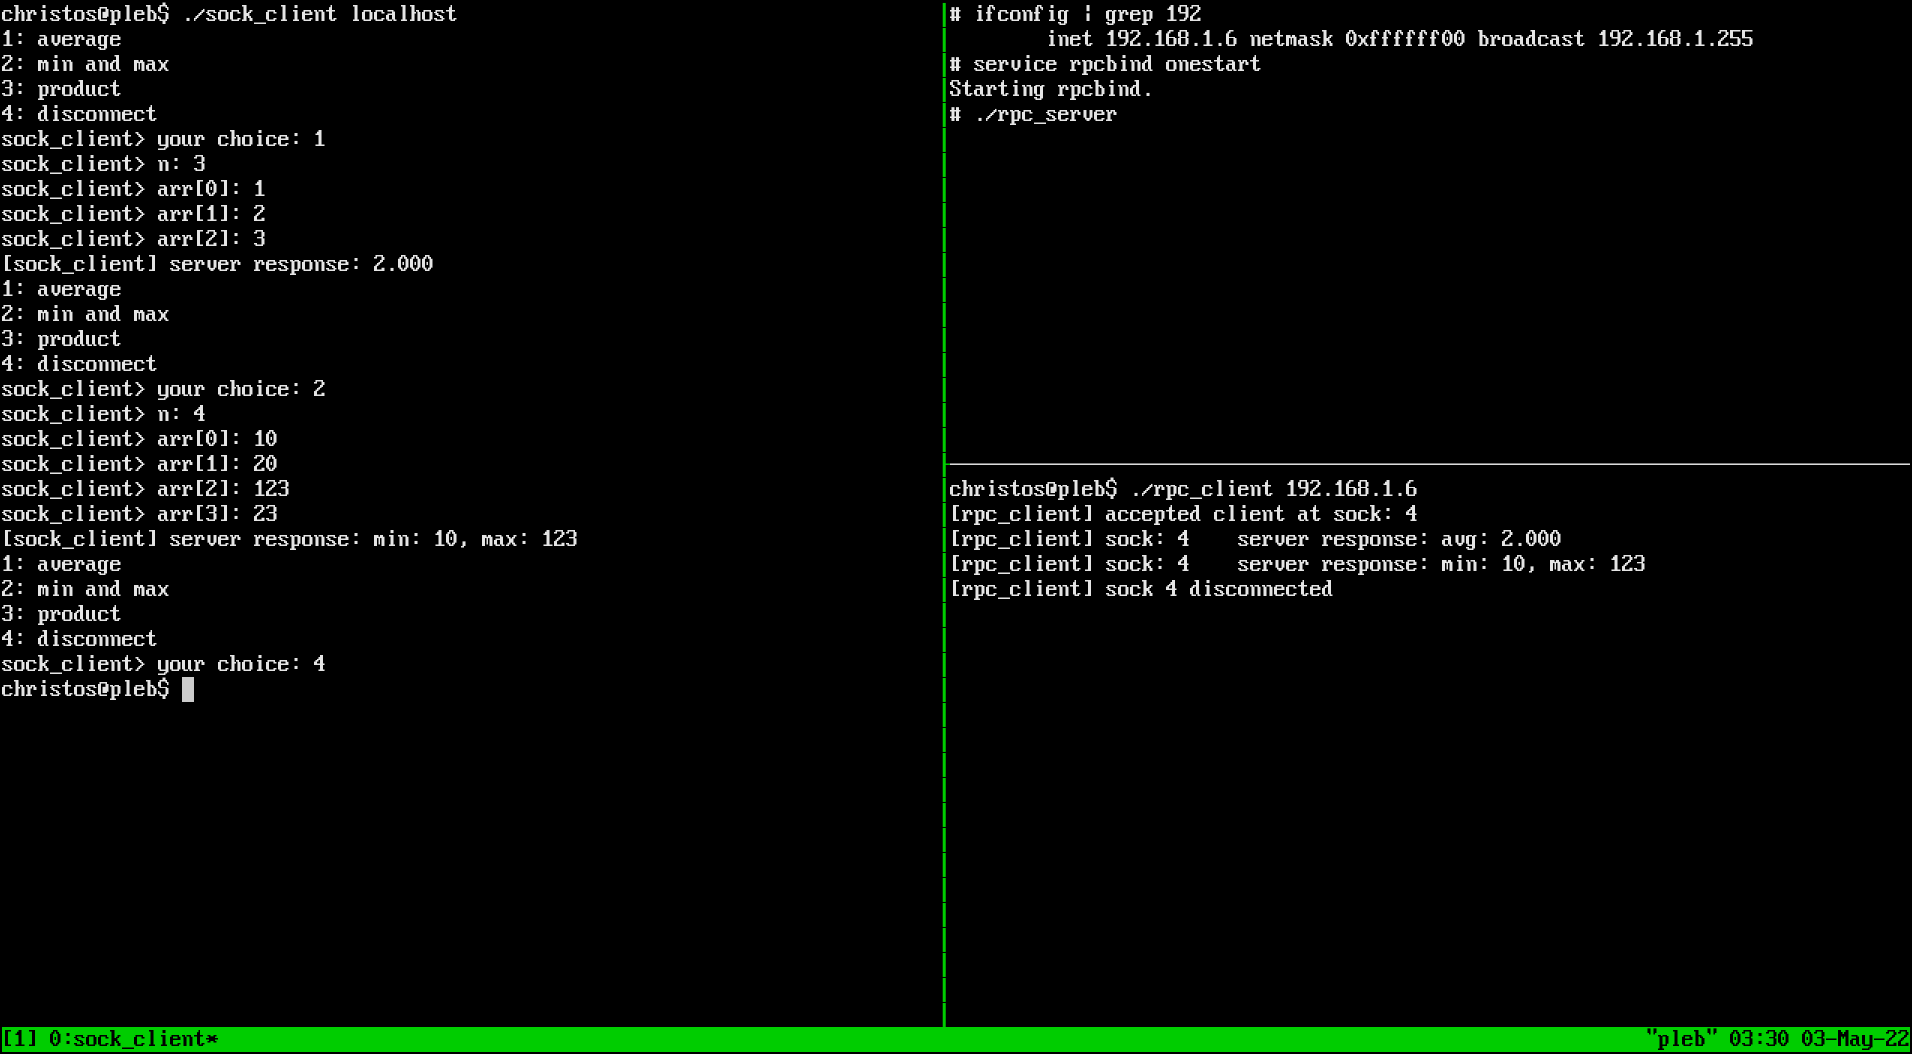
\includegraphics[width=\linewidth]{res/jail.png}

\subsection{Δοκιμή concurrency}

Ο RPC server και client τρέχουν και οι δύο σε FreeBSD Jail, και αυτή τη φορά θα
δοκιμάσουμε να ελέγξουμε αν ο server είναι όντως concurrent.

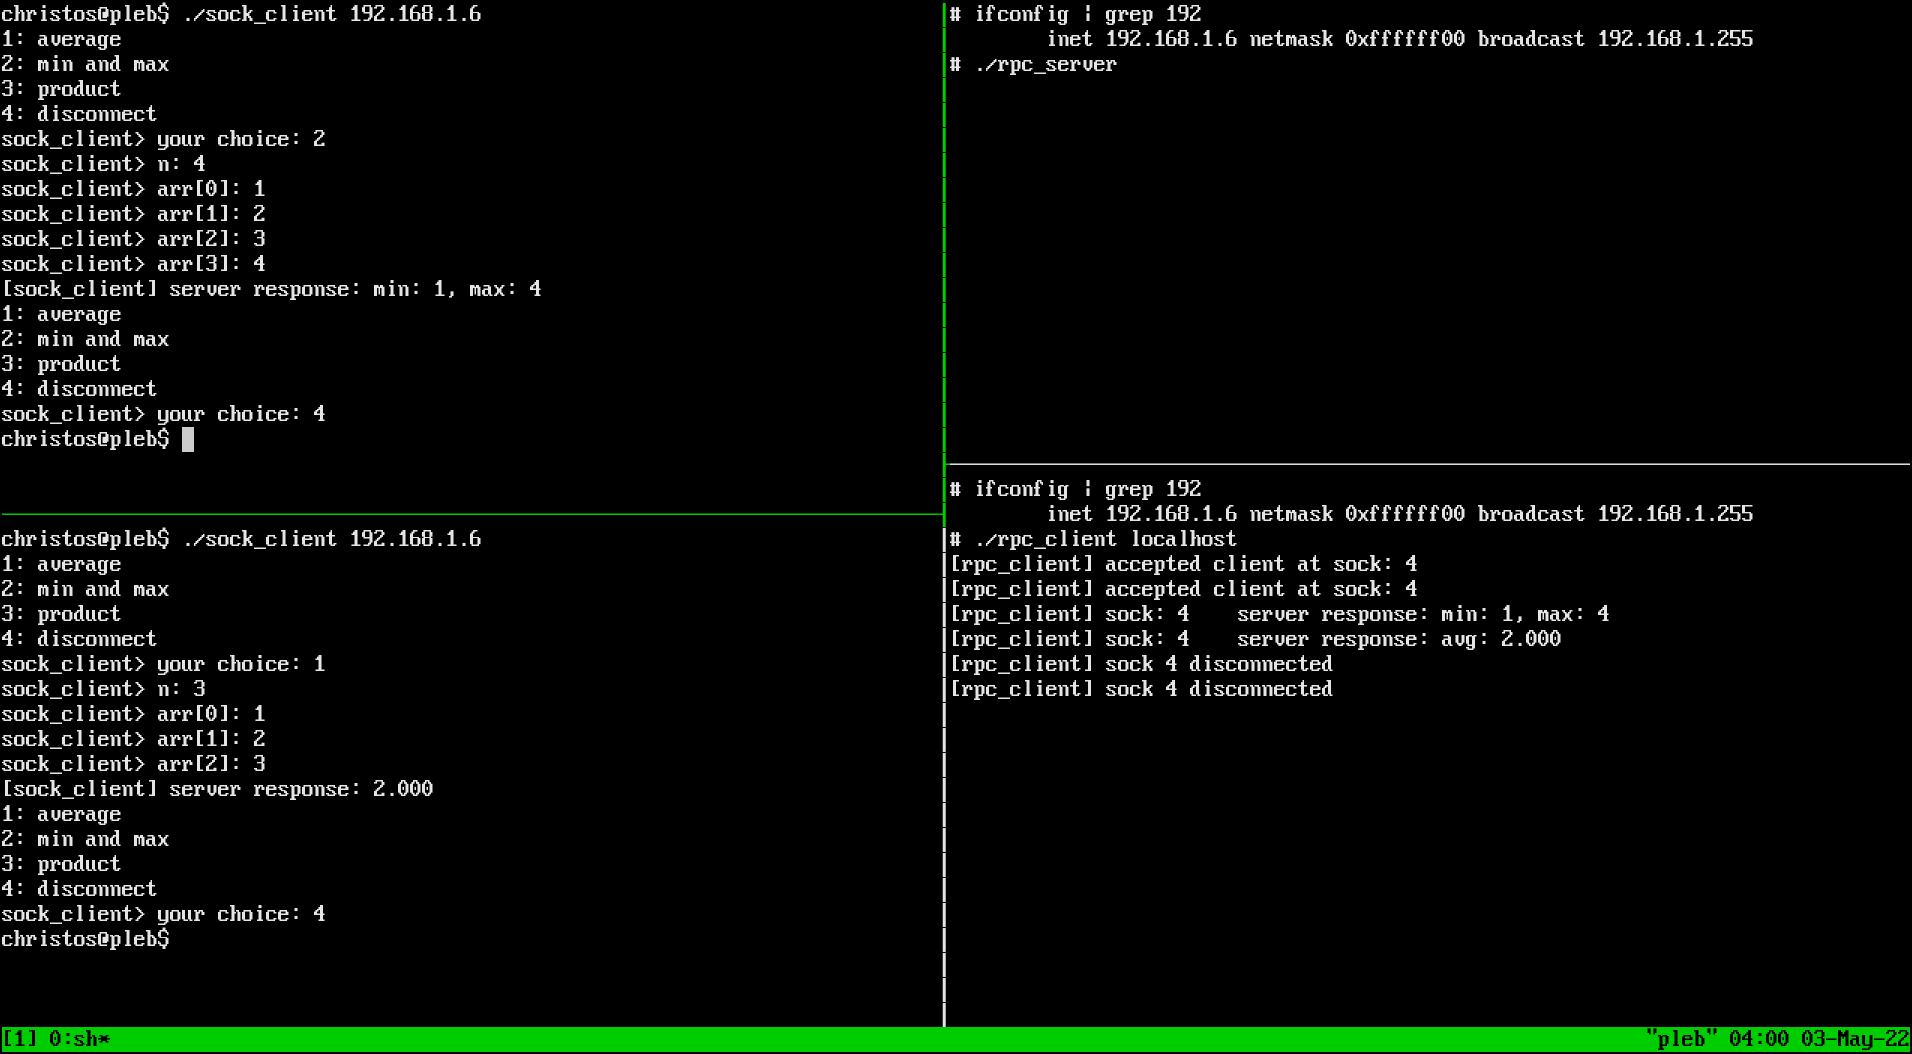
\includegraphics[width=\linewidth]{res/concur.png}

\section{Κώδικας}

Ο κώδικας είναι σχολιασμένος στα σημεία που θεωρώ ότι μπορεί να υπάρξει
σύχγηση, και όχι ακόμα και σε σημεία που είναι λίγο-πολύ ξεκάθαρο το τι
συμβαίνει.

\subsection{\lstinline{rpc.x}}

\lstinputlisting{../src/rpc.x}
\pagebreak

\subsection{\lstinline{rpc_server.c}}

\lstinputlisting[language=C]{../src/rpc_server.c}
\pagebreak

\subsection{\lstinline{rpc_client.c}}

\lstinputlisting[language=C]{../src/rpc_client.c}
\pagebreak

\subsection{\lstinline{sock_client.c}}

\lstinputlisting[language=C]{../src/sock_client.c}
\pagebreak

\subsection{\lstinline{Makefile.rpc}}

\lstinputlisting[language=make]{../src/Makefile.rpc}
\pagebreak

\subsection{\lstinline{Makefile}}

\lstinputlisting[language=make]{../src/Makefile}
\pagebreak

\end{document}
